% ****** Start of file apssamp.tex ******
%
%   This file is part of the APS files in the REVTeX 4.1 distribution.
%   Version 4.1r of REVTeX, August 2010
%
%   Copyright (c) 2009, 2010 The American Physical Society.
%
%   See the REVTeX 4 README file for restrictions and more information.
%
% TeX'ing this file requires that you have AMS-LaTeX 2.0 installed
% as well as the rest of the prerequisites for REVTeX 4.1
%
% See the REVTeX 4 README file
% It also requires running BibTeX. The commands are as follows:
%
%  1)  latex apssamp.tex
%  2)  bibtex apssamp
%  3)  latex apssamp.tex
%  4)  latex apssamp.tex
%
\RequirePackage{lineno}
\setlength{\linenumbersep}{6pt}

\documentclass[%
reprint,
%superscriptaddress,
%groupedaddress,
%unsortedaddress,
%runinaddress,
%frontmatterverbose, 
%preprint,
showpacs,preprintnumbers,
%nofootinbib,
%nobibnotes,
%bibnotes,
 amsmath,amssymb,
 aps,
%pra,
%prb,
%rmp,
%prstab,
%prstper,
%floatfix,
]{revtex4-1}

\usepackage{graphicx}% Include figure files
\usepackage{dcolumn}% Align table columns on decimal point
\usepackage{bm}% bold math
\usepackage{xspace}	% Include xspace
\usepackage{color}
\usepackage{xcolor}
\usepackage{amsmath}
%\usepackage{hyperref}% add hypertext capabilities
%\usepackage[mathlines]{lineno}% Enable numbering of text and display math
%\linenumbers\relax % Commence numbering lines

%\usepackage[showframe,%Uncomment any one of the following lines to test 
%%scale=0.7, marginratio={1:1, 2:3}, ignoreall,% default settings
%%text={7in,10in},centering,
%%margin=1.5in,
%%total={6.5in,8.75in}, top=1.2in, left=0.9in, includefoot,
%%height=10in,a5paper,hmargin={3cm,0.8in},
%]{geometry}

\newcommand{\pt}{\mbox{$p_T$}\xspace}
\newcommand{\raa}{\mbox{$R_{\rm AA}$}\xspace}
\newcommand{\raap}{\mbox{$R_{\rm AA}^{N_{\rm part}}$}\xspace}
\newcommand{\Npart}{\mbox{$N_{\rm part}$}\xspace}
\newcommand{\Ncoll}{\mbox{$N_{\rm coll}$}\xspace}
\newcommand{\Nch}{\mbox{$N_{\rm ch}$}\xspace}
\newcommand{\Et}{\mbox{${\rm E}_T$}\xspace}
\newcommand{\meanpt}{\mbox{$\langle p_T \rangle$}\xspace}
\newcommand{\meanet}{\mbox{$\langle {\rm E}_T \rangle$}\xspace}
\newcommand{\mNcoll}{\mbox{$\langle N_{\rm coll} \rangle$}\xspace}
\newcommand{\sqs}{\mbox{$\sqrt{s}$}\xspace}
\newcommand{\sqsn}{\mbox{$\sqrt{s_{_{NN}}}$}\xspace}
\newcommand{\dau}{\mbox{$d$+Au}\xspace}
\newcommand{\dpb}{\mbox{$d$+Pb}\xspace}
\newcommand{\pau}{\mbox{$p$+Au}\xspace}
\newcommand{\pal}{\mbox{$p$+Al}\xspace}
\newcommand{\hau}{\mbox{$^3\text{He}$+Au}\xspace}
\newcommand{\pp}{\mbox{$p$+$p$}\xspace}
\newcommand{\ppb}{\mbox{$p$+Pb}\xspace}
\newcommand{\pa}{\mbox{$p+A$}\xspace}
\newcommand{\rdau}{\mbox{$R_{dAu}$}\xspace}
\newcommand{\pda}{\mbox{$p(d)+A$}\xspace}
\newcommand{\rpda}{\mbox{$R_{p(d)+A}$}\xspace}
\newcommand{\bbceta}{\mbox{$3.0<|\eta|<3.9$}\xspace}

\bibliographystyle{unsrt}

\linenumbers

\begin{document}

\title{Measurement of Long-Range Angular Correlations and Azimuthal Anisotropies in High Multiplicity \pau Collisions at \sqsn = 200 GeV}% Force line breaks with \\

\author{Author list: Brant will insert later}

\date{\today}% It is always \today, today,
             %  but any date may be explicitly specified

\begin{abstract}
We present the first measurements of long-range angular correlations and the transverse momentum dependence of elliptic flow $v_2$ in high-multiplicity central \pau collisions at \sqsn = 200 GeV. A comparison of these results with previous measurements in central \dau and \hau collisions demonstrates a relation between $v_2$ and the initial collision eccentricity $\varepsilon_2$, suggesting that the observed azimuthal anisotropies in these small systems have a collective origin and reflect the initial geometry. Good agreement is observed between the measured $v_2$ and hydrodynamic calculations for all systems, disfavoring theoretical explanations based on momentum-space domain correlations. The set of measurements presented here provides the opportunity to leverage the distinct intrinsic geometry of each of these systems to distinguish between different theoretical descriptions of the long-range correlations observed in small collision systems. 
\end{abstract}

\pacs{25.75.Dw}% PACS, the Physics and Astronomy
                             % Classification Scheme.
%\keywords{Suggested keywords}%Use showkeys class option if keyword
                              %display desired
\maketitle
.\clearpage

The azimuthal momentum anisotropy of particle emission relative to the participant plane of the collision, as quantified by the Fourier coefficients $v_n$ of the final state particle yield, has long been considered evidence for the formation of a strongly interacting, fluid-like quark-gluon plasma (QGP) in A+A collisions~\cite{Heinz:2013th}. Viscous hydrodynamics supports a picture in which the initial spatial distribution in energy density, both from intrinsic geometry and fluctuations, is propagated into the final state as anisotropies in momentum space. The success of hydrodynamics in describing various bulk observables of the QGP has lent credence to the notion of hydrodynamic flow as the main driver of the $v_{n}$ signal in this class of collisions.

However, recent analyses of \dau and \hau collisions at \sqsn = 200 GeV~\cite{Adare:2015ctn,PhysRevLett.111.212301,Adamczyk:2014fcx,PhysRevLett.115.142301} at the Relativistic Heavy-Ion Collider (RHIC), and \ppb at \sqsn = 5.02 TeV, and $p+p$ at \sqsn = 7 and 13 TeV~\cite{alice_long_2013,atlas_observation_2012,cms_observation_2012,Khachatryan:2015lva,Aad:2015gqa,Khachatryan:2010gv,Khachatryan:2016txc} at the Large Hadron Collider (LHC) have demonstrated the existence of the same kind of azimuthal anisotropy signals commonly interpreted as evidence of collective behavior in larger systems. Notably, a feature known as \textit{the ridge} has been observed, consisting of a near-side (i.e., around $\Delta \phi = 0$) enhancement in the long-range (i.e., at large relative pseudorapidity) azimuthal two-particle correlation even after accounting for non-flow contributions. From these correlations, substantial elliptic ($v_2$), and triangular ($v_3$) flow coefficients are measured in these systems.

Although these observations seem to support the idea of QGP formation in small systems, it is not clear that hydrodynamic expansion would translate initial geometry into final state momentum anisotropy in this regime, where the formed medium is expected to be short-lived. Other explanations have been put forth, including initial state effects from glasma diagrams~\cite{dusling_azimuthal_2012}, color recombination~\cite{Ortiz:2013yxa}, and partonic scattering in transport models~\cite{bzdak_elliptic_2014,ma_long-range_2014,Koop:2015wea}. Transport model calculation, as well as those from hydrodynamics, involve the translation of initial geometry into momentum space via final state interactions. However, unlike in hydrodynamics where interactions involve fluid elements, transport models describe interactions between well defined particles in kinetic theory. In contrast, glasma diagrams take momentum-space domains as a starting point, resulting in momentum correlations without any final-state interactions. In this initial momentum-space domain picture, the correlations averaged over the event should become weaker in going from \pau, to \dau, to \hau as the average is taken over a larger number of domains, washing out the correlation effect. There is no correspondence to the geometry in this picture. A key experimental test to resolve the issue consists in varying the initial geometry of the system to analyze the extent to which it carries into the final state~\cite{nagle_exploiting_2013}.

The PHENIX collaboration has actively pursued this course of study by analyzing data from intrinsically elliptic (\dau)~\cite{Adare:2015ctn,PhysRevLett.111.212301} and triangular (\hau)~\cite{Adare:2015ctn} collision systems at \sqsn = 200 GeV. Viscous hydrodynamics followed by a hadron cascade has been found to accurately reproduce the measured $v_n$~\cite{Romatschke:2015gxa,adare_measurement_2014,PhysRevLett.111.212301,Adare:2015ctn,Bozek:2015qpa} for these systems.

This article completes the above suite of studies by presenting two-particle correlations and the transverse momentum (\pt) dependence of $v_2$ for central \pau collisions at \sqsn = 200 GeV. These results are compared to those from \dau and \hau collisions, as well as to available theoretical calculations. We apply the same analysis procedure on all three systems, on identical centrality selections, to provide a controlled comparison from which to draw conclusions.

A detailed description of the PHENIX detector can be found in Refs.~\cite{Adcox2003469,fvtx}. For this analysis, charged particles were reconstructed with the two central arm spectrometers, consisting of drift chambers (DC) and multi-wire proportional pad chambers (PC), each covering $|\eta|<0.35$ in pseudorapidity and $\pi/2$ in azimuthal angle. Drift chamber tracks are matched to hits in the third layer of the PC, thus limiting the contribution of tracks from decays and photon conversions. The beam-beam counters (BBC) comprise two arrays of 64 quartz radiator \v{C}erenkov detectors, located longitudinally $\pm$1.44 m away from the center of the interaction region (IR), covering \bbceta and 2$\pi$ in azimuth. The forward vertex detector (FVTX) is a silicon detector comprising two identical end-cap assemblies symmetrically located in the longitudinal direction around the IR, covering the pseudorapidity range $1.0 < |\eta| < 3.0$. It uses hit clusters to detect charged particles with an efficiency greater than 95\%.
The arms of the BBC and FVTX in the Au-going direction (i.e., direction of negative pseudorapidity) are designated as the \emph{south} arms and styled BBC-S and FVTX-S, respectively. We use each of these two detectors to determine the flow event plane. In addition, the $z$-vertex of the collision is found using information from both arms of the BBC. In this analysis, a $\pm$30 cm event vertex cut was applied for \pp, and a ,$\pm$10 cm cut for \pau.

The \pau data set for this analysis was collected during the 2015 data-taking run at RHIC. It consists of 0.84 billion minimum bias (MB) triggered events and 1.4 billion high-multiplicity (HM) triggered events. The MB trigger is defined as a coincidence in the same event between the BBC detectors in the Au-going and $p$-going directions, requiring at least one photomultiplier tube (PMT) firing in each; in this way 84$\pm$4\% of the total inelastic \pau cross section is captured. The HM trigger is based on the MB trigger, but imposes the additional requirement of more than 48 photomultiplier tubes firing in the BBC-S. 

In this analysis, we select the 0\%-5\% most central \pau events, where 
centrality classes are defined by the quantiles of the total multiplicity measured in the BBC-S, following the procedure documented in Ref.~\cite{bbc}.
The initial geometry of events in these centrality selections is characterized using a standard Monte Carlo Glauber approach, where nucleon coordinates are smeared by a Gaussian of width $\sigma = 0.4$ fm. In this model, initial state eccentricity $\varepsilon_2$ is computed from initial nucleon coordinates, as shown in Eq.~\ref{eqn:epsilon2}. 

\begin{equation}
\label{eqn:epsilon2}
\varepsilon_2 = \frac{\sqrt{\langle r^2\cos (n\phi)\rangle ^2 + \langle r^2\sin (n\phi) \rangle ^2}}{\langle r^2 \rangle}
\end{equation}

\begin{table}
\caption{Geometric characterization of small system collisions at \sqsn = 200 GeV in the 0\%-5\% centrality class, using Monte Carlo Glauber with nucleon coordinates smeared by a two-dimensional Gaussian of width $\sigma=0.4$ fm.}
\begin{ruledtabular}
\begin{tabular}{c c c c}
\label{table_geometry}
 & \pau (0\%-5\%) & \dau (0\%-5\%) & \hau (0\%-5\%) \\
\hline
 $\langle N_{coll} \rangle$ & $9.7\pm 0.6$ & $18.1\pm 1.2$ & $26.1\pm 2.0$ \\
 $\langle N_{part} \rangle$ & $10.7\pm 0.6$ & $17.8\pm 1.2$ & $25.1\pm  1.6$ \\ 
 $\langle \varepsilon_2 \rangle$ & $0.23\pm 0.01$ & $0.54\pm 0.04$ & $0.50\pm 0.02$
\end{tabular}
\end{ruledtabular}
\end{table}

The results of this characterization are shown in Table~\ref{table_geometry}. Long-range angular correlations are constructed between charged tracks in the PHENIX central arms at a given \pt, and charge deposited in the BBC-S PMTs, for central \pau collisions. The distribution of these track-PMT pairs is constructed over relative azimuth as given in Eq.~\ref{eq31}, with the normalized correlation function given by Eq.~\ref{eq:def_corr_function}, following Ref.~\cite{PhysRevLett.115.142301}:
\begin{eqnarray}
  S(\Delta\phi,p_{T})=
  \frac{ d(w_{{\rm PMT}} N^{{\rm track}(p_{T}){\rm - PMT}}_{{\rm Same \; event}}) }{ d\Delta\phi}, & &
\label{eq31} \\
  C(\Delta\phi,p_{T}) =
          \frac{S(\Delta\phi,p_{T})}{M(\Delta\phi,p_{T})} \:
          \frac{\int_{0}^{2\pi} M(\Delta\phi,p_{T}) \, d\Delta\phi}{\int_{0}^{2\pi} S(\Delta\phi,p_{T}) \, d\Delta\phi}. & &
  \label{eq:def_corr_function}
\end{eqnarray}
The weights $w_{{\rm PMT}}$ for each pair correspond to the charge in the PMTs. The signal distribution $S$ is constructed from pairs in the same event. The mixed distribution $M$ is constructed using pairs from different events in the same centrality class and collision vertex bin.

%%%%%%%%%%%%%%%%%%%%%%%%%%%%  Fig_1 %%%%%%%%%%%%%%%%%%%%%%%%%
% figure showing BBC-S-CNT correlations
\begin{figure*}[htbp]
  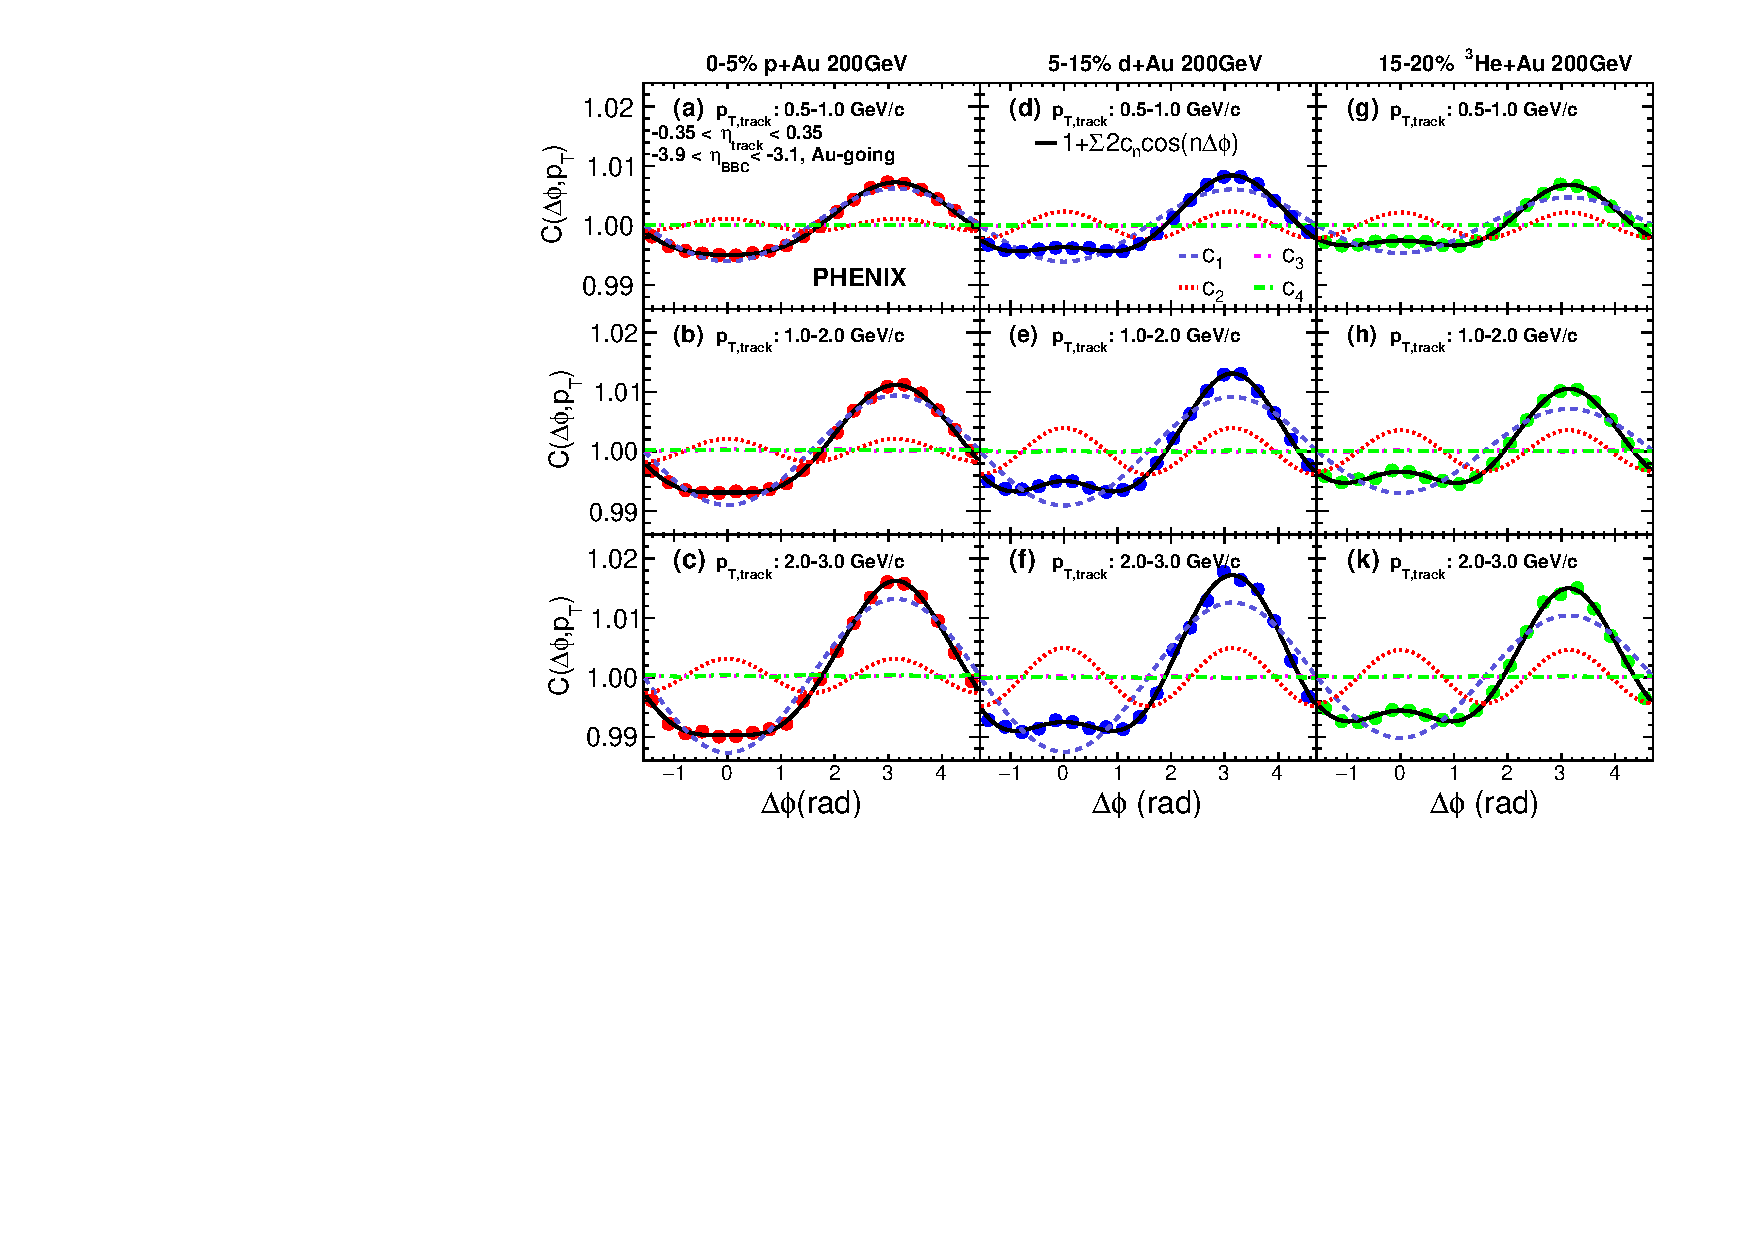
\includegraphics[scale=0.8]{Figures/figure1.pdf}
  \caption{(Color online) Long-range angular correlations $C(\Delta\phi,p_{T})$ constructed with central arm tracks and BBC-S PMT pairs, in 0\%--5\% central \pau collisions at \sqsn~=~200~GeV. From left to right,
correlations are shown for various track \pt categories: (a) 0.5--1.0 GeV/$c$, (b) 1.0--2.0 GeV/$c$, and (c) 2.0--3.0~GeV/$c$. We fit each correlation with a four-term cosine Fourier series; individual harmonics shown as dashed lines, and the total fit is shown as a solid line.}
\label{fig:figure1}
\end{figure*}

%%%%%%%%%%%%%%%%%%%%%%%%%%%%  Fig_2 %%%%%%%%%%%%%%%%%%%%%%%%%
% figure showing c2 coefficients
\begin{figure}[htbp]
  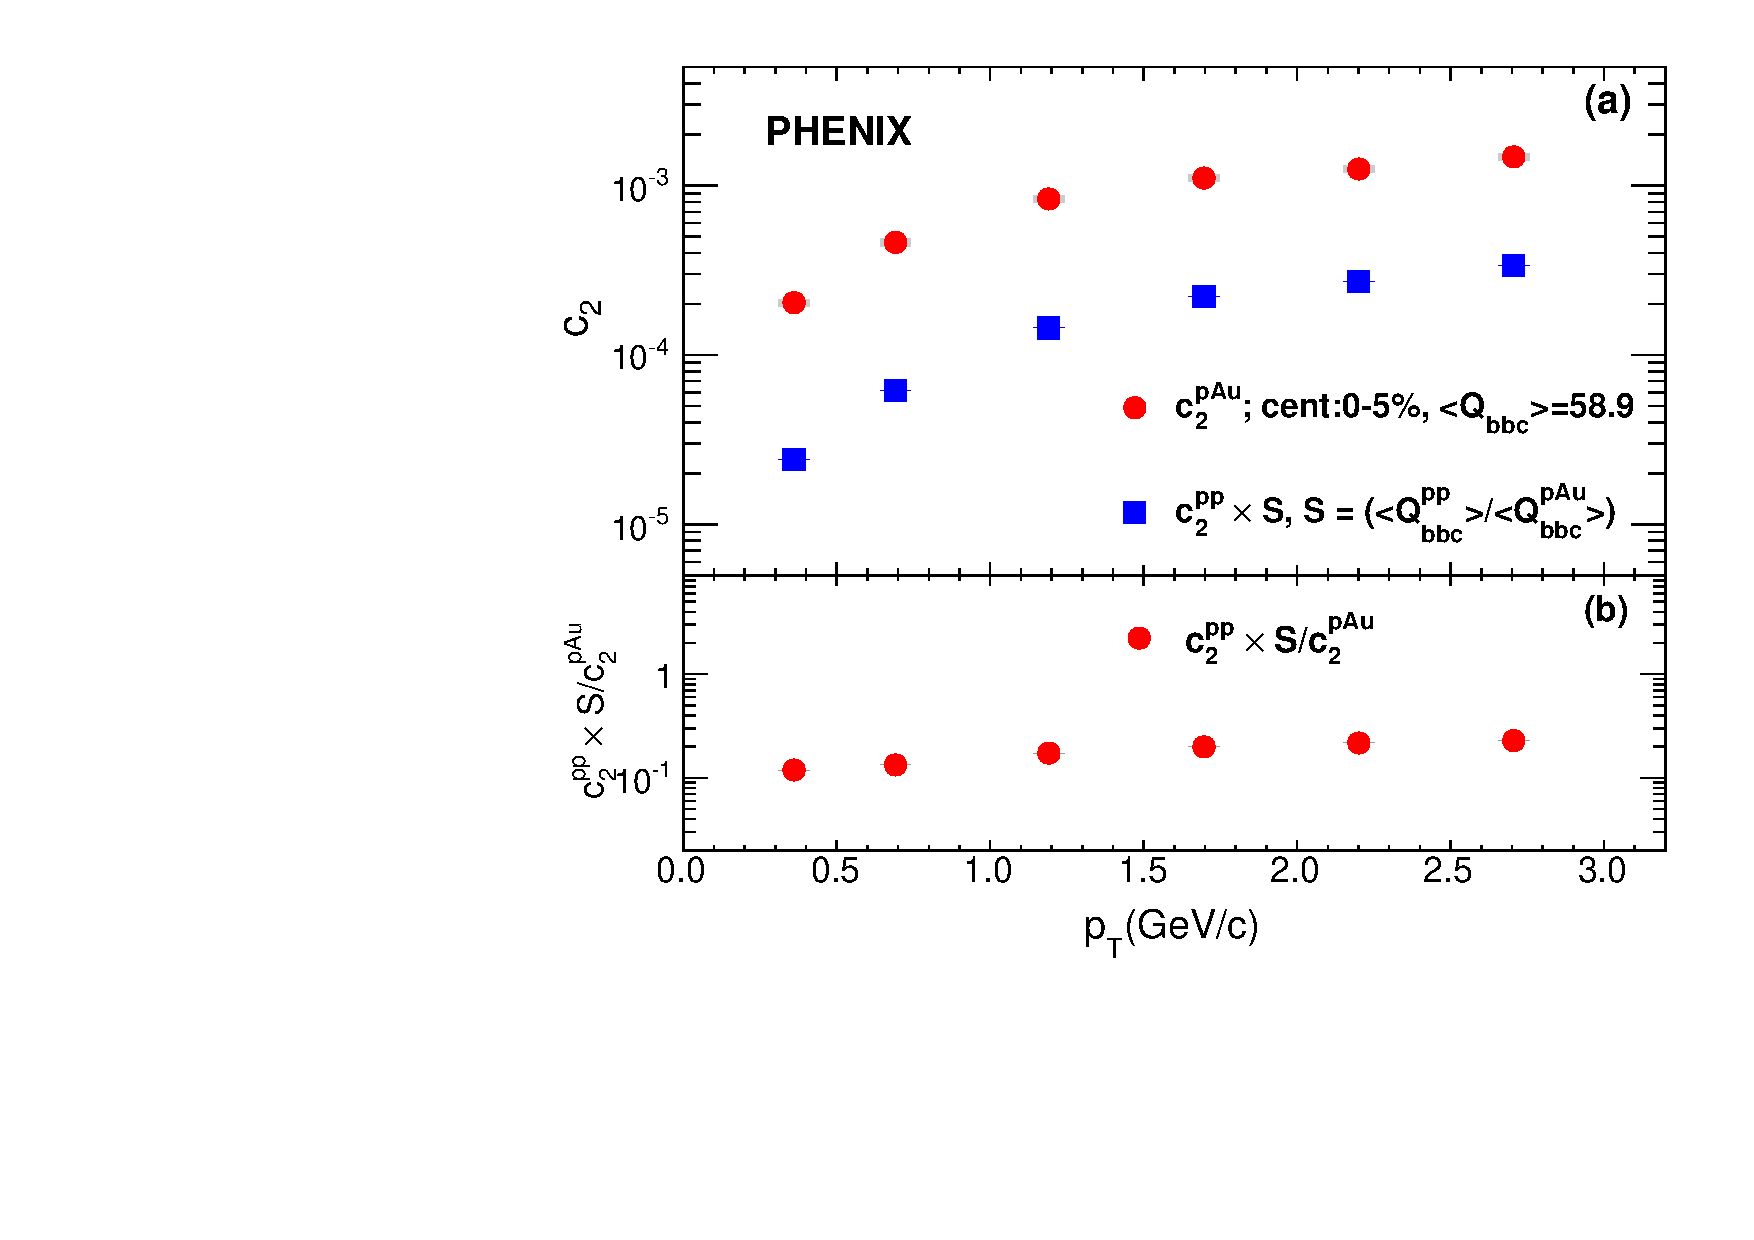
\includegraphics[scale=0.45]{Figures/figure2.pdf}
  \caption{(Color online)~The second order harmonic coefficients $c_2(p_T)$ for long range angular correlations in
0\%--5\% \pau collisions, as well as for minimum bias \pp collisions. The latter are scaled down by the factor $\left( \sum Q^{{\rm BBC-S}} \right)_{p+p} / \left( \sum Q^{{\rm
BBC-S}} \right)_{{\rm pAu}}$. (b)~The
ratio of the two harmonics is plotted with the corresponding statistical errors.
}
\label{fig:figure2}
\end{figure}

The resulting correlation functions for three track \pt selections are shown in Figure ~\ref{fig:figure1}. Each one is fit with a four-term cosine Fourier series. The magnitude of the second harmonic ($c_{2}$) as a function of \pt is shown with red circles in Fig.~\ref{fig:figure2} panel (a). The contribution of elementary processes (e.g., jet fragmentation, resonance decays, and momentum conservation effects) to the measured $c_2$ in \pau can be estimated quantitatively using previously published $c_2$ from \pp at the same collision energy~\cite{Adare:2015ctn}, scaled down by an appropriate factor to account for the higher multiplicity in \pau. We choose the scale factor to be the ratio of the total charge deposited in the BBC-s in \pp relative to \pau, as shown in Eq.~\ref{eq:dilute}. 

\begin{equation}
c_{n}^{{\rm pAu \; elementary}}(p_{T}) \simeq c_{n}^{p+p}(p_{T})
\frac{\left( \sum Q^{{\rm BBC-S}} \right)_{p+p}}
{\left( \sum Q^{{\rm BBC-S}} \right)_{{\rm pAu}}
}.
\label{eq:dilute}
\end{equation}

The scaled down reference $c_{2}$ is shown with blue squared in Fig.~\ref{fig:figure2}, panel (a). The ratio of $c_2$ in \pau to the scaled-down \pp reference is shown in panel (b). From this ratio, it can be seen that the relative correlation strength in \pau from elementary processes is at most 23\% at the highest \pt. Since this procedure constitutes an approximation to quantify the non-flow correlation strength, we do not subtract it from the total signal, treating it instead as a source of systematic uncertainty.

It is noteworthy that, unlike in \dau~\cite{adare_measurement_2014} and \hau~\cite{PhysRevLett.115.142301} collisions at the same centrality, the long-range angular correlations in \pau do not exhibit a discernible near-side peak, yet possess a non-negligible second harmonic component. Additionally, it is observed that the relative contribution of elementary processes to the total correlation strength $c_2$ is much higher in \pau, being more than twice the value quoted for the other two systems using the same \pp reference. The absence of a visible near-side peak can be understood in terms of the lower multiplicity of these p+Au events. Non-flow effects from jet correlations, for example, involve a finite number of particles, and are suppressed in events with higher multiplicity.

Having quantified the strength of the correlations from elementary processes, we determine the second Fourier coefficient $v_2$ of the single-particle azimuthal distributions, which is typically associated with collective elliptic flow, using the event plane method as described in Ref.~\cite{Poskanzer:1998yz}. Namely, we measure 

\begin{equation}
v_{2}(p_{T}) = \frac{\langle \cos 2(\phi_{\text{Particle}}(p_{T})-\Psi^{\text{FVTX-S}}_{2})\rangle}{\text{Res}(\Psi^{\text{FVTX-S}}_{2})}
\end{equation}
for charged hadrons at midrapidity, where the second order event plane $\Psi^{FVTX-S}_{2}$ is determined for every event using the FVTX-S detector. Its resolution is computed using the standard three-subevent method, correlating measurements in the BBC-S, FVTX-S, and the central arms. This results in $\text{Res}(\Psi^{\text{FVTX-S}}_{2})$ = 0.171. It is also possible to measure the event plane using the BBC-S. In that case, we obtain a lower resolution $\text{Res}(\Psi^{\text{BBC-S}}_{2})$ = 0.062, and $v_2$ values that differ from the FVTX-S measurement by approximately 3\%. The very good agreement of $v_2$, as measured using the BBC-S and FVTX-S event planes, is interesting since the pseudorapidity gaps relative to the midrapidity tracks are $|\Delta\eta| > 2.65$ and $|\Delta\eta| > 0.65$, respectively.

The main sources of systematic uncertainty in the $v_2(p_T)$ measurement are: (1) track background from photon conversion and weak decays, whose magnitude we estimate at 2\% relative to the measured $v_2$, by varying the spatial matching windows in the PC3 from 3$\sigma$ to 2$\sigma$; (2) multiple collisions per bunch crossing (i.e., event pile-up) that are estimated to occur  at an average rate of 8\% in the 0\%-5\% central p+Au collisions. Low luminosity and high-luminosity subsets of the data were analyzed separately and the systematic uncertainty in the $v_2(p_T)$ value is estimated to be asymmetric  +4\%-0\%, since the v2  values were found to decrease in the events that contain a larger fraction of pile-up; (3) non-flow correlations from elementary processes that enhance the $v_2$ values, whose contribution we estimate from Fig.~\ref{fig:figure2}, thus assigning a \pt-dependent asymmetric uncertainty with a maximum value of $^{+0}_{-23}\%$ for the highest \pt bin; (4) the asymmetry between the east ($\pi/2 < \phi < 3\pi/2$) and west ($-\pi/2 < \phi < \pi/2$) acceptance of the detectors due to an offset of 3.6 mrad between the colliding beams and the longitudinal axis of PHENIX, necessary for running \pau at the same momentum per nucleon. We applied a corresponding counter-rotation to every central arm track and detector element in the FVTX and BBC, which were also reweighted to restore their uniformity in azimuth. We estimate this systematic uncertainty at 5\% by taking the difference of $v_2$ as measured independently in the east and the west arms after applying the above corrections; (5) the difference in the $v_2(p_T)$ values when measured independently using the BBC-S and FVTX event planes, which we observe to be 3\%. 

\label{s:sys}
%%%%%%%%%%%%%%%%%%%%%%%%%%%%%%%% Systematic Table %%%%%%%%%%%%%%%%%%%%%%%%%%%%%%%%%%%%
\begin{table}[htbp]
  \begin{center}
    \begin{tabular}{ccc}
      \hline
      \hline
      Source& Systematic Uncertainty & Type \\ \hline
      Track Background &2.0\%& A\\ 
      Event Pile-up    &$^{+0}_{-4}\%$& B\\
      Non-Flow    &$^{+0}_{-23}\%$& B\\
      Beam Angle &5.0\%& C\\  
      Event-Plane Detectors & 3\% & B\\
    \hline
    \hline
    \end{tabular}
   \caption{\label{t:sys}Systematic uncertainties given as a percent of the $v_2$ measurement. Note that the non-flow contribution is expected to be \pt dependent and the value here quoted corresponds to the highest \pt.}
   \end{center}
 \end{table}

Table~\ref{t:sys} summarizes of all these systematic
uncertainties, categorized by type:

(A) point-to-point uncorrelated between $p_T$ bins,

(B) point-to-point correlated between $p_T$ bins,

(C) an overall normalization uncertainty in which all points are scale by the same multiplicative factor.

The resulting $v_2$ measurement for \pau, compared to \dau and \hau in the same 0\%-5\% centrality class, is shown in Fig.~\ref{fig:figure3}. In all cases, there is a substantial $v_2$ that rises with \pt. It is notable that the $v_2$ values for \dau and \hau are consistent within uncertainties, as are their eccentricities listed in Table I. The \pau collisions have a significantly lower $v_2$ and a correspondingly lower calculated $\varepsilon_2$. At the same time, the ordering of $v_2$ from \pau, to \dau, to \hau also follows the expected increasing order of particle multiplicity. In the case of \dau and \hau, for the 0\%-5\% most central events, the midrapidity charged particle density is published as $dN_ch/d\eta$ = 20.8 +/- 1.5 and 26.3 +/- 1.8 respectively~\cite{Adare:2015bua}. Fig.~\ref{fig:figure3} also shows $v_2$ calculations for each system from the \textsc{sonic}~\cite{Habich:2014jna} hydrodynamic model, matched to the multiplicity of our centrality selections, generating its initial conditions from the identical Monte Carlo Glauber simulation used to characterize event geometry. In all cases, a good agreement is seen within uncertainties between the data and the calculation. These observations strongly support the notion of initial geometry, coupled to the hydrodynamic evolution of the medium as a valid framework to understand small system collectivity.

To further explore this idea, we divide the $v_2$ curves by their corresponding $\varepsilon_2$ from Table~\ref{table_geometry}, attempting to establish a scaling relation between the two quantities. Figure~\ref{fig:figure4} shows that the ratios do not collapse to a common value. This behavior is also reproduced by the \textsc{sonic} calculation, as expected since both data and calculation are divided by the same $\varepsilon_2$ values. The lack of scaling in the \textsc{sonic} calculation can be understood from \dau events where the neutron and proton from the deuteron projectile are far separated and create two hot spots upon impacting the Au nucleus. These events have a large $\varepsilon_2$, but can result in small $v_2$ if the two hot spots evolve separately, never combining with the hydrodynamic time evolution. This effect is present in the \dau and \hau systems, and lowers the average $v_2/\varepsilon_2$ as detailed in Ref.~\cite{nagle_exploiting_2013}. 

\begin{figure}[htbp]
  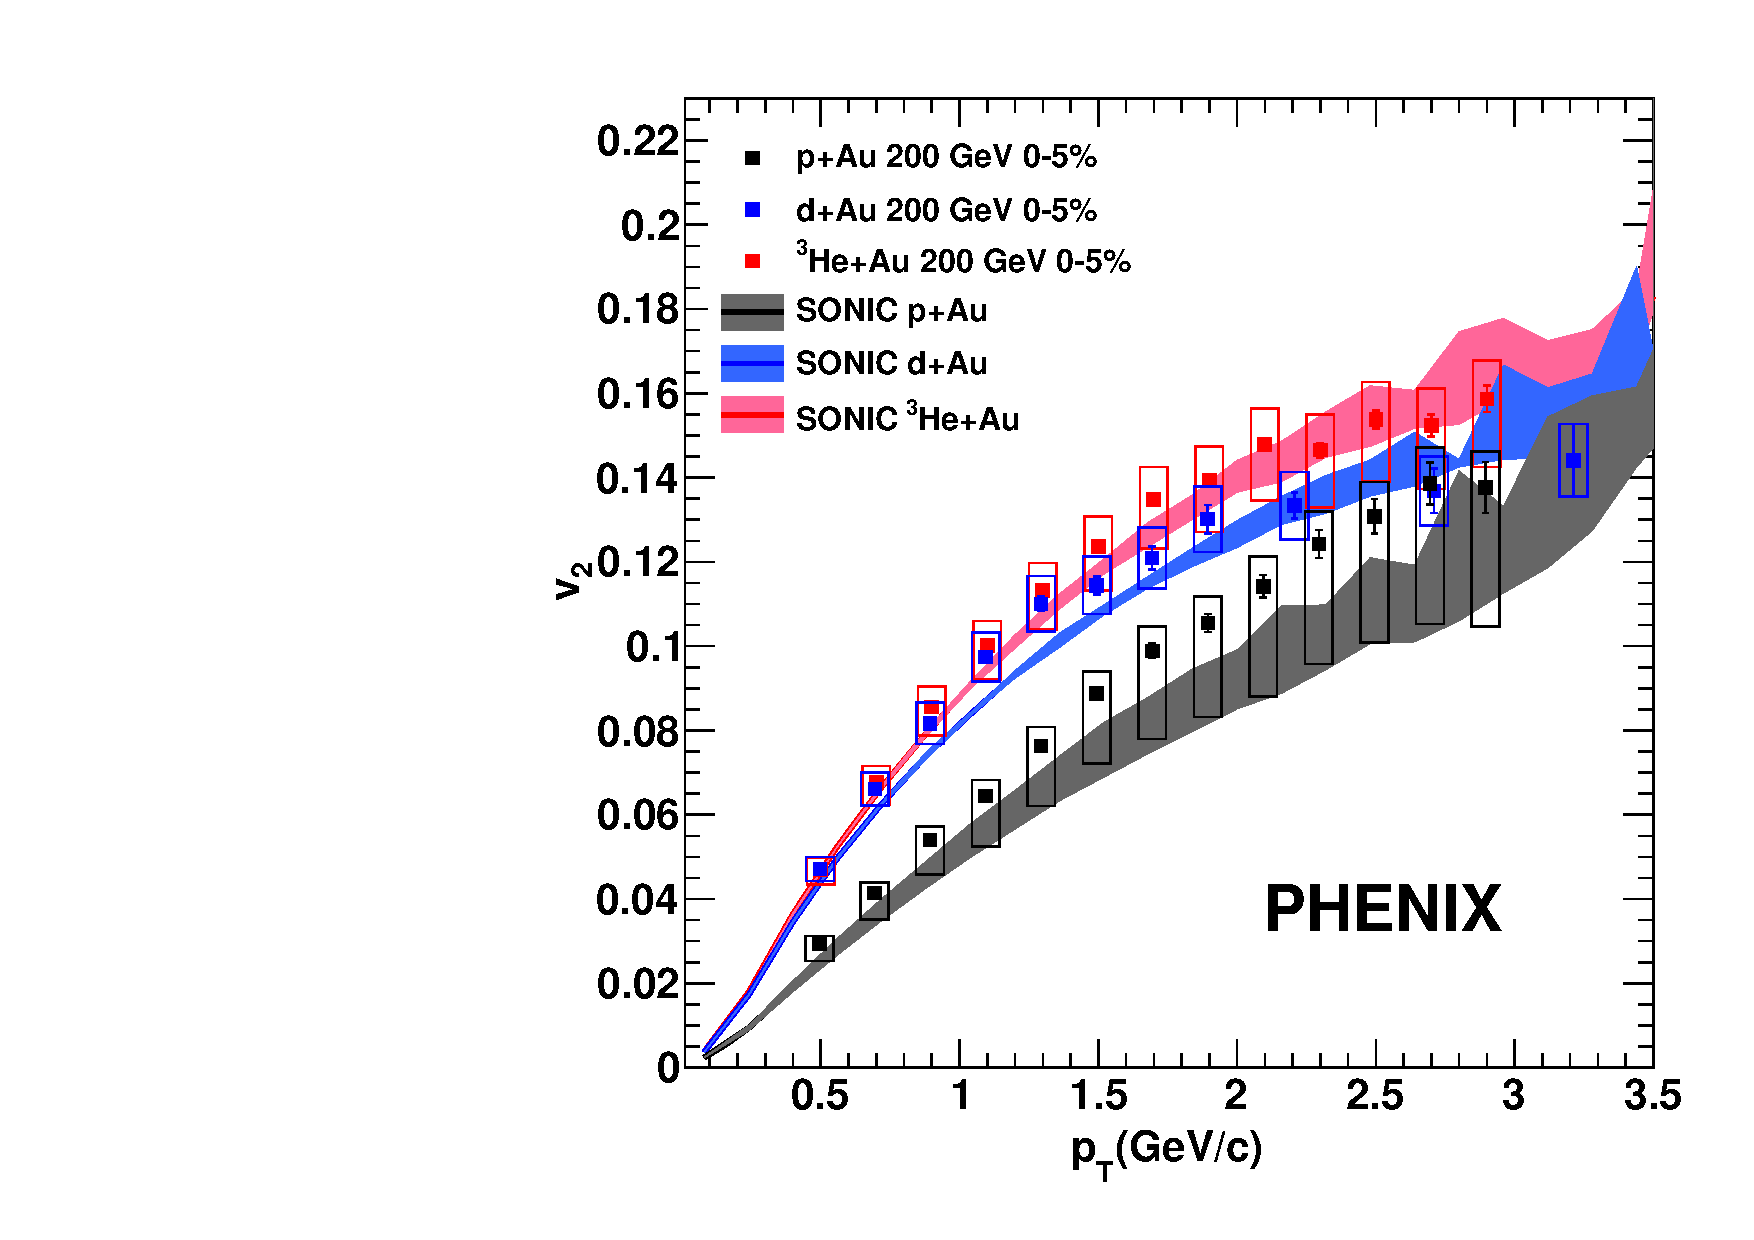
\includegraphics[scale=0.45]{Figures/figure3.pdf}
  \caption{(Color online) $v_2$ of charged hadrons within $|\eta| <$ 0.35 in 0\%--5\% \pau, \dau, and \hau central collisions, compared to hydrodynamic calculations using the \textsc{sonic} model, matched to the same multiplicity as the data.}
\label{fig:figure3}
\end{figure}

\begin{figure}[htbp]
  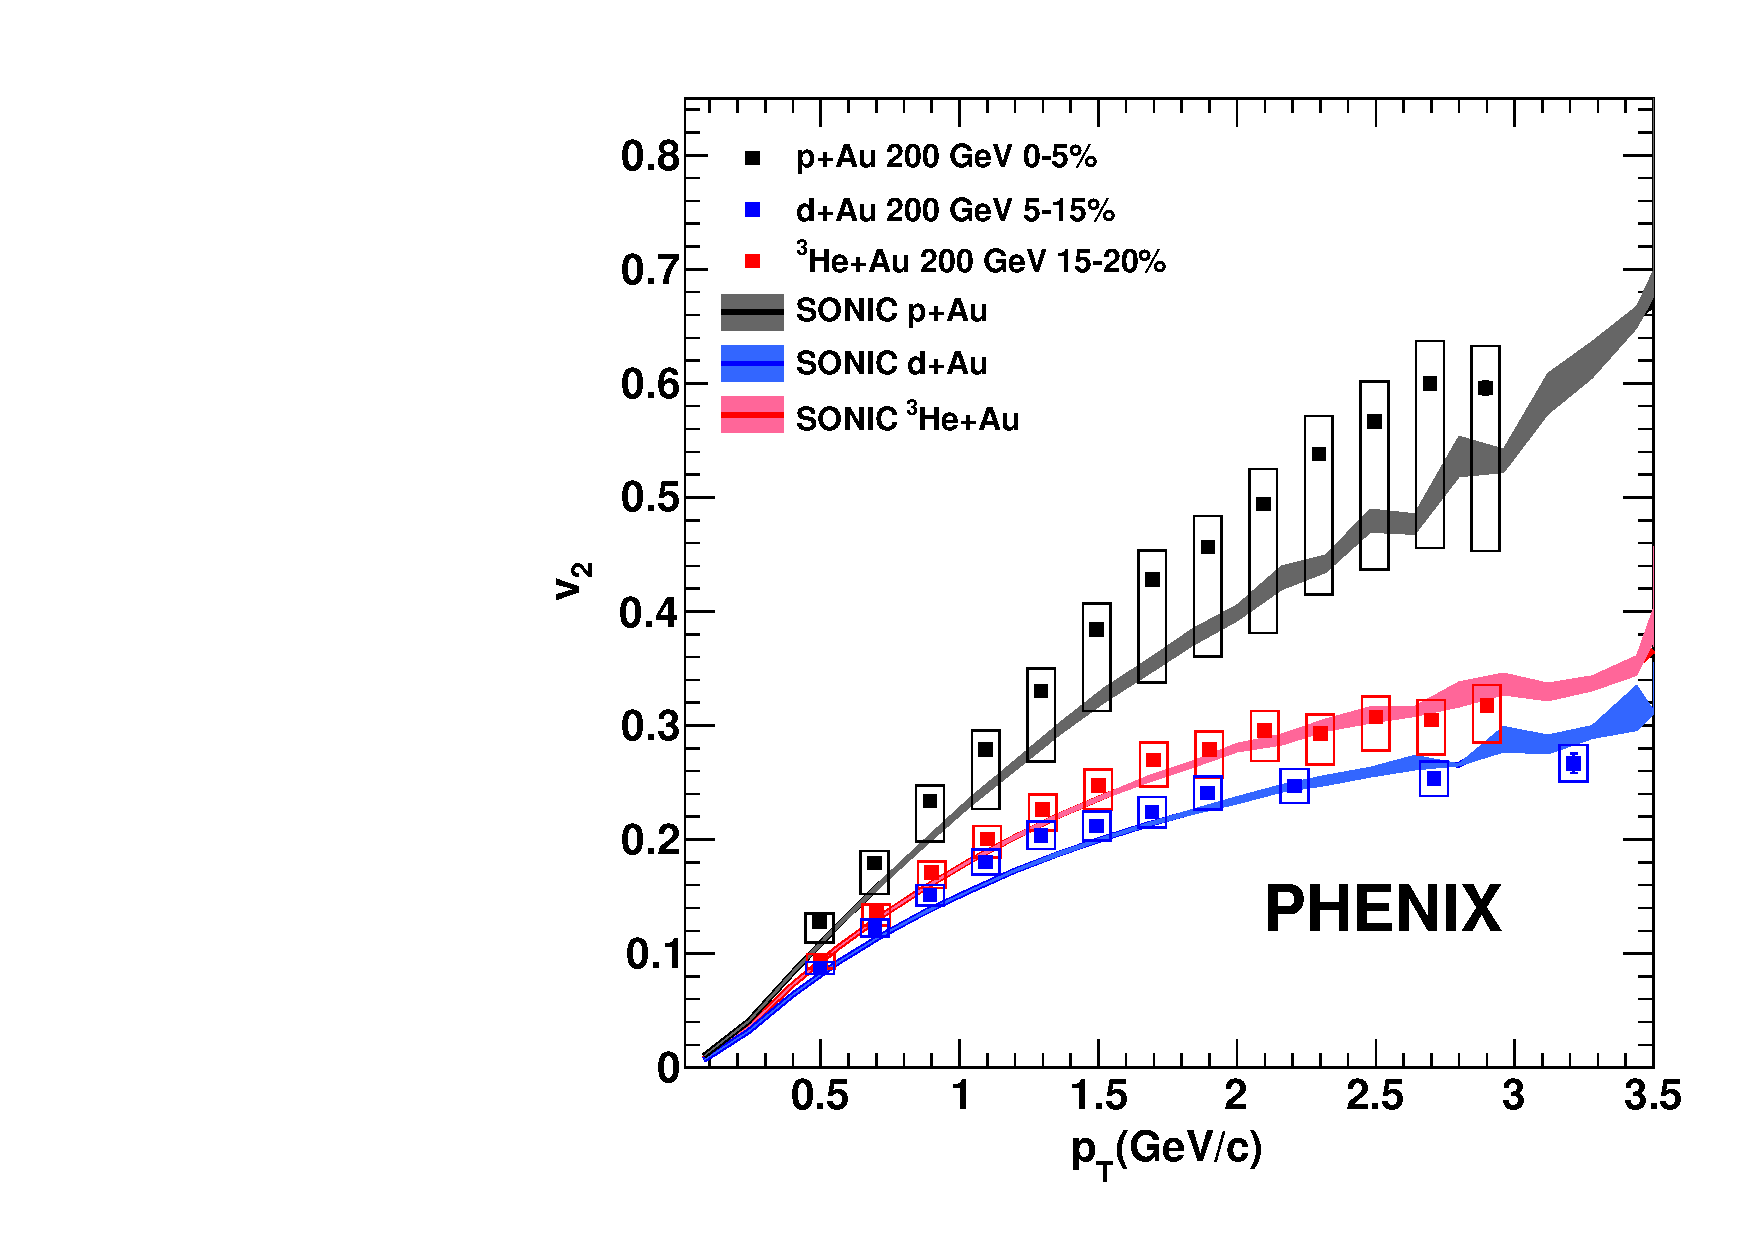
\includegraphics[scale=0.45]{Figures/figure4.pdf}
  \caption{(Color online) $v_2$ of charged hadrons within $|\eta| <$ 0.35 in 0\%--5\% \pau, \dau and \hau central collisions, divided by their corresponding eccentricity $\varepsilon_2$ from Glauber calculations, compared to \textsc{sonic} calculations of the same quantity.}
\label{fig:figure4}
\end{figure}

Figure~\ref{fig:figure5} shows $v_2(\pt)$ for 0\%-5\% central \pau, \dau, and \hau events, along with theoretical predictions available in the literature, most notably from hydrodynamics with Glauber initial conditions (\textsc{sonic}~\cite{Habich:2014jna} and \textsc{supersonic}~\cite{Romatschke:2015gxa}), hydrodynamics with IP-Glasma initial conditions~\cite{Schenke:2014gaa}, and A-Multi-Phase-Transport Model (\textsc{ampt})~\cite{lin_multiphase_2005}.

\begin{figure*}[htbp]
  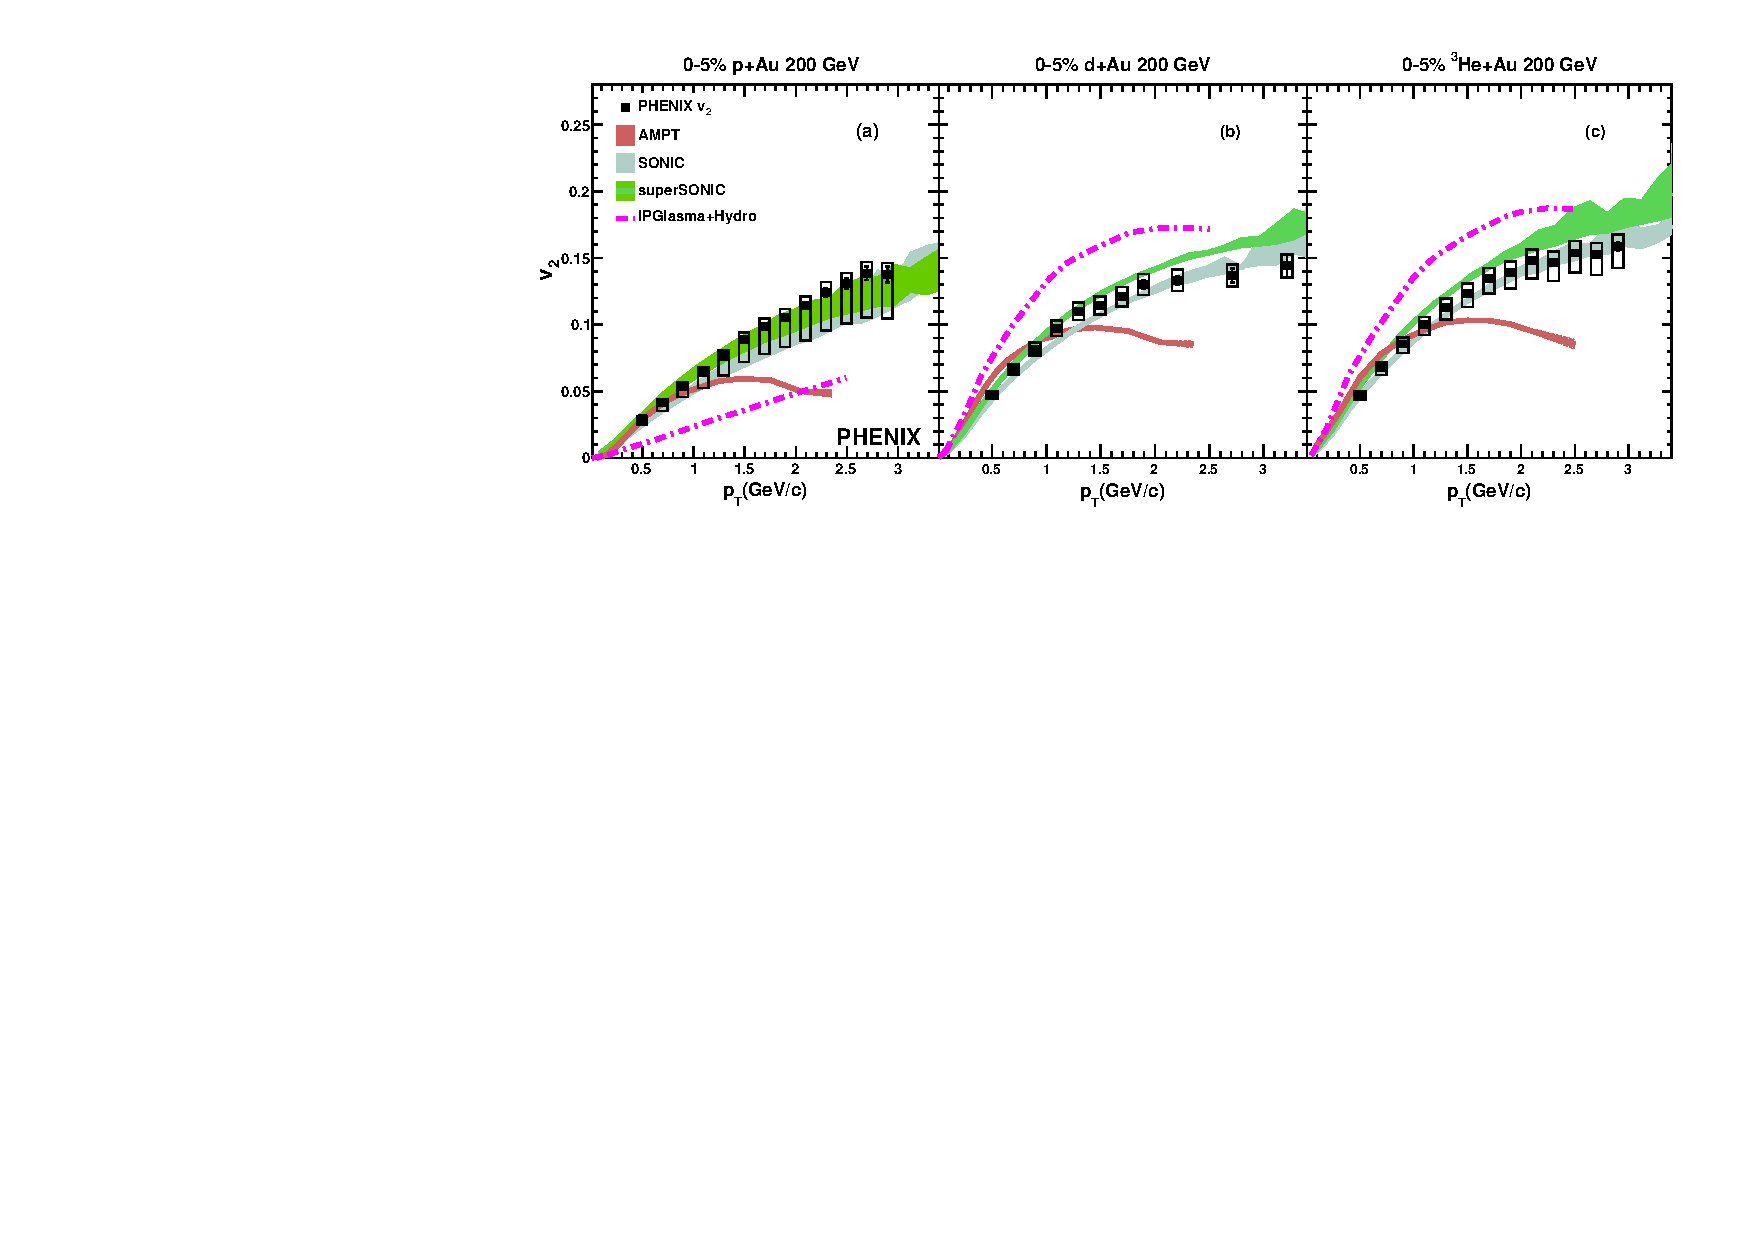
\includegraphics[scale=0.9]{Figures/figure5.pdf}
  \caption{(Color online) Transverse momentum dependence of $v_2$ in central 0\%-5\% (a) \pau, (b) \dau, and (c) \hau collisions at \sqsn = 200 GeV. Theoretical calculations from \textsc{ampt}, \textsc{(super)sonic}, and IPGlasma+Hydro are shown in each panel.}
\label{fig:figure5}
\end{figure*}

The \textsc{sonic} and \textsc{supersonic} models incorporate standard Monte Carlo Glauber initial conditions followed by viscous hydrodynamics, and a transition to a hadronic cascade at T = 170 MeV. Additionally, \textsc{supersonic} incorporates pre-equilibrium dynamics with a calculation in the framework of the AdS/CFT correspondence~\cite{vanderSchee:2013pia,Chesler:2015wra,Romatschke:2013re}. These two models agree well with the data within uncertainties, supporting the idea of initial geometry as the driver of the $v_n$ signal. Furthermore, this illustrates how these results impose useful constraints to reduce the number of \emph{free parameters} of the model, since many such parameters must be identical across systems, e.g., $\eta/s$, the transition temperature to a hadron cascade, and the  Monte Carlo Glauber smearing of nucleon coordinates of $\sigma=0.4$ fm.

Predictions using IP-Glasma initial conditions followed by viscous hydrodynamics substantially overestimate the data for \dau and \hau, while underestimating it for \pau. This follows from the fact that IP-Glasma generates very \emph{circular} initial conditions for \pau, corresponding to very low $\varepsilon_2$ values; however, the presence of several hot spots in \dau and \hau result in IP-Glasma values for $\varepsilon_2$ more comparable to those from Glauber. This is shown in Table~\ref{table_geometry_glasma}. 

\begin{table}[h!]
\caption{Geometric characterization of small systems at \sqsn = 200 GeV for 0\%-5\% centrality from IP-Glasma initial conditions, and Monte Carlo Glauber initial conditions smeared with a two-dimensional Gaussian of width $\sigma=0.4$ fm.}
\begin{ruledtabular}
\begin{tabular}{c c c c}
\label{table_geometry_glasma}
 & \pau & \dau & \hau \\ \hline
 Glauber $\langle \varepsilon_2 \rangle$ & $0.23\pm 0.01$ & $0.54\pm 0.04$ & $0.50\pm 0.02$ \\
 IP-Glasma $\langle \varepsilon_2 \rangle$ & $0.10\pm 0.02$ & $0.59\pm 0.01$ & $0.55\pm 0.01$ \\
\end{tabular}
\end{ruledtabular}
\end{table}

In the case of \dau and \hau, a better agreement with data can be achieved by increasing the value of $\eta$/s or by including a hadronic cascade stage. However, doing so would lower the prediction for \pau even further. This demonstrates that IP-Glasma does not generate the appropriate initial conditions to account for measured $v_n$ via hydrodynamic flow. 

It is important to notice that additional degrees of freedom on the geometry of \pau collisions arise from fluctuations of the shape of the proton, as described in Ref.~\cite{Schlichting:2014ipa}. The contribution of this effect to the measured elliptic flow may be constrained by $p+p$ data, and also possibly by varying the target in other $p+$A systems.

Finally, \textsc{ampt} combines partonic and hadronic scattering in a single model. Using the initial Glauber geometry information to compute $v_2$ relative to the participant plane~\cite{Koop:2015wea} yields results that agree reasonably well with the data below $\pt \approx 1$ GeV/c, yet underpredict them at higher \pt. It is noteworthy that despite the very different physics of \textsc{ampt} compared to the other models, it has successfully been applied to a variety of systems at RHIC and the LHC. See, for example, Refs.~\cite{Adare:2015cpn,Koop:2015wea,Ma:2016fve,ma_long-range_2014,ma_long-range_2014}

We have presented results on azimuthal anisotropy and elliptic flow in central \pau at \sqsn = 200 GeV, compared with $v_2$ in \dau and \hau collisions. These results impose strong constraints on any model attempting to describe small system collectivity, whether by the formation of strongly interacting hot nuclear matter, or other mechanisms. We observe an imperfect scaling of $v_2$ with $\varepsilon_2$, well reproduced by hydrodynamics, providing strong evidence for initial geometry as the source of final-state momentum anisotropy in these systems. This disfavors other explanations based on initial-state momentum space domain effects. Further insight into the nature of small system collectivity can be gained by analyzing the centrality and collision energy dependence of $v_2$, and will be the subject of future studies. 

\bibliography{references}
\end{document}
%
% ****** End of file apssamp.tex ******